\chapter{Discussion}\label{sec:discussion}

In this chapter, we discuss advantages and disadvantages of the different 
models developed in this thesis and competitor models, justifying contributions 
of this thesis.  Performance of the different models in terms of part 
localization accuracy is in ~\secref{system-results}.

\section{The case for image-dependent interactions}

At the time of publication, CPS was significantly better than all modern ``in 
the wild'' pose estimation approaches 
\citep{ferrari08,eichner09,devacrf,andriluka09}.  CPS was the only one to use 
image-dependent pairwise cues.  These other systems focused on either 
pre-processing to reduce the state space or improving unary potentials via 
foreground color estimation, and all performed inference relying ultimately on 
edge-based unary potentials and simple geometric displacement pairwise cues as 
in the classical PS model (\secref{ps}).


Recently, \citet{deva2011} introduced a multi-modal model of pose that competes 
with CPS. However, empirical results indicate that CPS generalizes better than 
\citet{deva2011}---both models applied to the Pascal dataset were trained on 
Buffy.  Furthermore, two years after its introduction in the literature, CPS is 
still the best performing model in the less precise regime 
(\figref{results-buffy-pascal}).  One of the reasons for the lack of precision 
is the coarser nature of our features: whereas \citet{deva2011} can evaluate 
placements to the granularity of a HoG cell, many of our features are more 
coarsely described and/or discretized---\eg, is the part guess near a contour, 
is the part guess in the foreground color.

In a more controlled setting, we see that a classical PS model coupled with 
just one image-dependent interaction feature---contour 
continuity---significantly improves performance (\figref{ablative}).

The benefits of image-dependent interactions is further reinforced by the 
performance by our video pose estimation model.  The Ensemble of Stretchable 
Models exploits a variety of across-body and across-frame image interactions 
and significantly outperfoms methods with fewer interactions.

In general, our cascade approach is a principled framework that frees us from 
restricting our models to simplified pairwise potentials of the form 
$\phi_{ij}(y_i - y_j)$. This allows much more flexibility in the future 
incorporating more pairwise and even higher-order features. 

\section{More features or more modes?}
As first mentioned in~\secref{llps}, there are two major approaches for 
improving pose accuracy in recent years: adding more features, \eg CPS, ESM and 
\citet{ferrari08,eichner09,ddtran}, or adding more modes, \eg LLPS and 
\citet{dpm,wang2011,deva2011,johnson11}.  

Currently, LLPS slightly underperforms CPS and~\citet{deva2011}.  However, it 
ambitiously uses an order of magnitude more modes than existing multi-modal 
approaches.  It may be suffering due the computational difficulties preventing 
joint training of different modes, and lack of a sufficiently sized dataset.  
\figref{llps-learning-curve} indicates further improvement with larger 
datasets.

\begin{figure}[htb!]
\centering
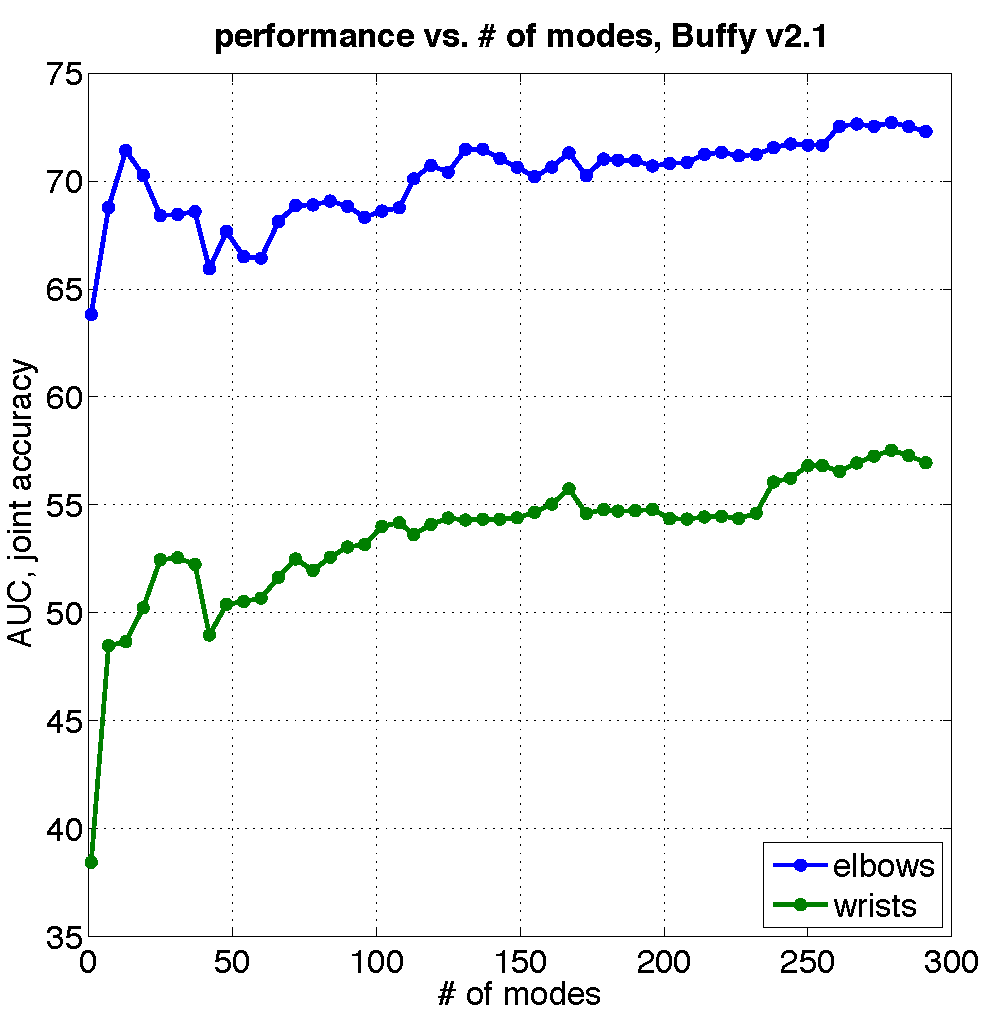
\includegraphics[width=0.59\linewidth]{figs/llps-learning-curve.pdf}
\caption[Test accuracy versus number of local neighborhood modes in LLPS.]{
\label{fig:llps-learning-curve} We show test set accuracy on Buffy for LLPS, 
measured by area under the joint precision curve.  For this analysis, we added 
modes to our model in the order they were chosen by our greedy mode selection 
process / basis pursuit (\secref{calib}).  We stopped at the point 
cross-validation determined there were no more beneficial modes to add. The 
increasing performance as a function of number of modes implies that having a 
larger training set with more local neighborhoods would further improve 
accuracy of our system.  It is important to note that training and inference 
scale linearly (and are parallelizable) with the number of modes in our method, 
so we intend to investigate this for future work.}
\end{figure}


Ultimately, these research directions are complementary, and an ideal model 
would use a combination of rich features and multiple modes. Additional feature 
types (\eg, segments, contours, optical flow, depth) incurs an additional cost 
to obtain, but adds to the generalization capabilities of the model. Additional 
modes allows for more specific modeling of different scenarios, but requires 
more training data to estimate parameters accurately.  This leaves a large 
space of possible models combining the two approaches.

\section{Joints or limbs?}

\section{Detection, localization, or both?}

\section{Everything and the kitchen sink: a bug or a feature?}
One of the main contributions of this thesis was technical contributions that 
allow us to include a veritable kitchen sink of features---the goal was to 
include as many feature modalities as possible in our CPS and ESM models.  
Having so many features makes it difficult to determine exactly what is 
contributing to the success of our model.  From a machine learning standpoint, 
this is an attractive aspect of our system: given training data, we can try 
everything and see what works.  From a computer vision standpoint, this is a 
disadvantage---it is difficult to gain insight into why the model is performing 
well exactly.


\section{Accuracy, speed, simplicity}
time vs accuracy vs complexity

\chapter{Future directions}

what will it take to work?
  + more data
  + more computation

does the right cost function exist?

\chapter{Conclusion}

This thesis proposes advancements in 2D human pose estimation models to improve 
upon state-of-the-art performance.  Specifically, previously proposed pictorial 
structures models are handicapped by the needs of efficient inference tricks; 
forced to express simple pairwise cues that are only a function of parts' 
spatial relationships.  Further, the spatial relationship structure had to form 
a tree graph.

We push past the inference barrier in several ways, allowing us to include 
richer image-dependent interactions.  First, we proposed Cascaded Pictorial 
Structures, a sequence of structured models that efficiently prune the state 
space of possible poses down to a manageable number.  This allows us to perform 
efficient exact inference without restrictions.  We exploit this by 
incorporating a variety of rich features from complementary sources, improving 
upon state-of-the-art PS approaches in single frame pose estimation.

We then extend this approach to handle pose estimation in video.

Finally, LLPS.

We show empirically that we are awesome.

Future.

The end.










